% Finite State Machine (Automaton)
% Demonstrates: TikZ automata library for DFA/NFA diagrams.
% Compile with: pdflatex main.tex

\documentclass[border=10pt]{standalone}
\usepackage{tikz}
\usetikzlibrary{automata, positioning, arrows.meta}

\begin{document}
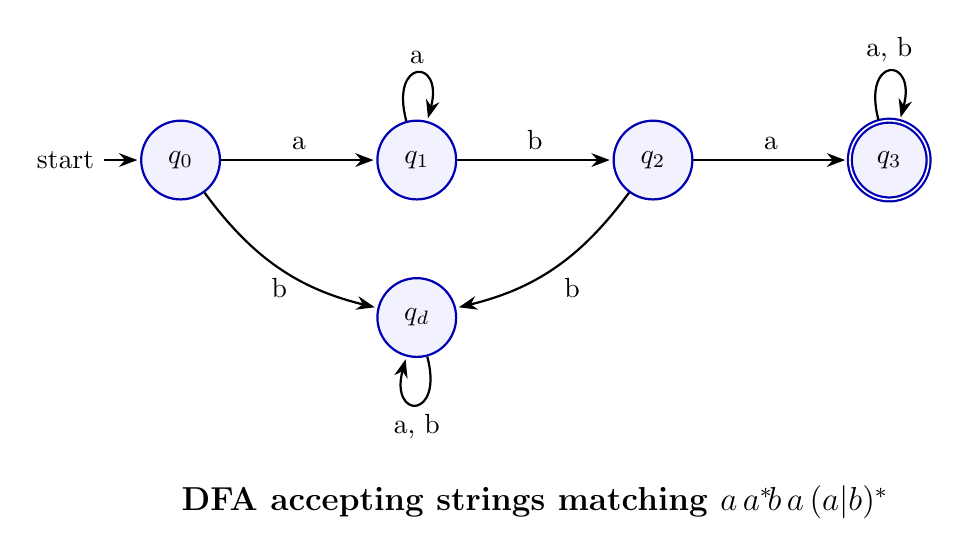
\begin{tikzpicture}[
    ->,
    >=Stealth,
    shorten >=1pt,
    node distance=3cm,
    on grid,
    auto,
    thick,
    every state/.style={
        draw=blue!70!black,
        fill=blue!5,
        minimum size=1cm,
        font=\normalsize,
    },
]

% --- States ---
\node[state, initial]           (q0) {$q_0$};
\node[state]                    (q1) [right=of q0] {$q_1$};
\node[state]                    (q2) [right=of q1] {$q_2$};
\node[state, accepting]         (q3) [right=of q2] {$q_3$};
\node[state]                    (qd) [below=2cm of q1] {$q_d$};

% --- Transitions ---
\path
    (q0) edge                   node {a}     (q1)
    (q0) edge [bend right=20]   node [below] {b}     (qd)
    (q1) edge                   node {b}     (q2)
    (q1) edge [loop above]      node {a}     ()
    (q2) edge                   node {a}     (q3)
    (q2) edge [bend left=20]    node {b}     (qd)
    (q3) edge [loop above]      node {a, b}  ()
    (qd) edge [loop below]      node {a, b}  ()
;

% --- Label ---
\node[anchor=north, font=\large\bfseries] at (4.5, -4) {
    DFA accepting strings matching $a\,a^*\!b\,a\,(a|b)^*$
};

\end{tikzpicture}
\end{document}
